%%%%%%%%%%%%%%%%%%%%%%%%%%%%%%%%%%%%%%%%%%%%%%%%%%%%%%%%%%%%%%%%%%%%%%%%%%%%%%%%%%
%%																				%%
%% File name: 		00sarah.tex													%%
%% Project name:	Hochleistungsantenne										%%
%% Type of work:	T3X00 project work											%%
%% Author:			Sarah Brückner, Maximilian Stiefel, Hannes Bohnengel		%%
%% Date:			27th Arpil 2016												%%
%% University:		DHBW Ravensburg Campus Friedrichshafen						%%
%% Comments:		Created in gedit with tab width = 4							%%
%%																				%%
%%%%%%%%%%%%%%%%%%%%%%%%%%%%%%%%%%%%%%%%%%%%%%%%%%%%%%%%%%%%%%%%%%%%%%%%%%%%%%%%%%
%\cite{kauffels}\newpar

\chapter{Projektmanagement}
Schon Thomas Carlyle (1795–1881) erkannte die Wichtigkeit von strukturierten und organisiertem Vorgehen als er sagte:\newpar
``Unsere Hauptaufgabe ist nicht, zu erkennen, was unklar in weiter Entfernung liegt, sondern zu tun, was klar vor uns liegt''.\newpar
In einem Projekt ist das strukturierte und organisierte Vorgehen der klare Weg zu einem 
erfolgreichem Ziel. Daher wird sich in dieser Arbeit
dem Projektmanagement bedient um die Antennennachführung für Satelliten in die richtige Richtung zu 
lotsen. Dabei lehnt sich das Management an 
das bekannte V-Modell, welche den Ablauf von Software-, als auch von Hardwareentwicklungsprozessen 
beschreibt. Dieses Modell soll einem Projekt 
die Richtung weisen, jedoch werden die einzelnen Schritte vom Projektmanager selbst definiert. Ein 
Vorhersagemodell wie dieses legt folgende
Prozesse fest:
\begin{itemize}
 \item die Aktivitäten die durchzuführen sind,
 \item die Reihenfolge des Arbeitsablaufes,
 \item die Definition von Ergebnissen,
 \item die Fertigstellungskriterien,
 \item die Ressourcen die vorhanden sind
 \item und die anzuwendenden Standards/Werkzeuge.
\end{itemize}
\begin{figure}[h]
 \centering
 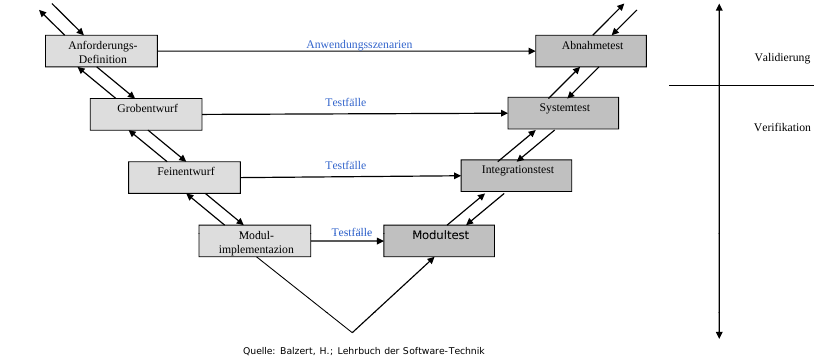
\includegraphics[width=0.8\linewidth]{./images/vmodell}
 \caption{V-Modell, Quelle: \cite{swscript}} %Universität Leipzig, Softwaretechnik}
 \label{fig:vmodell}
\end{figure}
Eine wichtige Rolle spielt die Qualitätssicherung, die das V-Modell sicher stellt. In diesem Modell sind die Verifikation und die Validation ein 
fester Bestandteil. Verifikation bedeutet, die Sicherstellung dass das entwickelte Produkt mit den Spezifikationen übereinstimmt.
Die Validation ist die Eignung des Produkts bezogen auf seinen Einsatzzweck. Durch die Sicherstellung beider Qualitätsmerkmale wird das Projekt 
erfolgreich zu seinem Ziel, die Antnennennachführung für Satelliten, geführt.Aus diesem Grund ist 
das V-Modell die richtige Vorgehensweise für 
dieses Projekt.
\newpar

\section{Zeitplan}
Bevor ein Projekt starten kann, ist wichtig  zu definieren, wie viel Zeit für die Durchführung zu Verfügung steht. Für diese Studienarbeit 
wird drei Studierenden einen Zeitrahmen von zwei Semerster zugeschrieben. Dafür sind pro Studenten 300 Stunden kalkuliert. Beginn der Studienarbeit 
ist der 14. Oktober 2015 und endet am 15. Juli 2016. Für die Studierenden der Kurse TEN, TEK und TLE 
ist im Stundenplan jeder Mittwoch von 14 Uhr bis 
17.15 Uhr Studienarbeitszeit vorgesehen. Dies ist eine grobe Richtlinie für die Durchführung der Studienarbeit und kann nach Bedarf angepasst werden.
\newpar

\section{Anforderungsdefinition}
Implementierung einer quelloffenen, kostenfreien Software zur Antennennachführung für das Verfolgen 
von erdnahen Satelliten. Die zur Antennennachführung
benötigten Schnittstellen werden von der Hochschule zur Verfügung gestellt und sollen für diese Arbeit verwendet werden. Die Software soll die 
Satellitenposition mit Hilfe der Keplerelemente und den Doppler-Shift berechnen und ausgeben. Die Ausgabe soll grafisch erfolgen und anzeigen, wann
der gewählte Satellit verfügbar ist. Ist der gewählte Satellit verfügbar, soll die Antenne in die richtige Position nachgeführt werden. 
\newpar

\section{Arbeitspakete}
Arbeitspakete brechen das Projekt in einzelne Aufgaben runter und werden an einen 
zuständigen Mitarbeiter zugeteilt. Ein Arbeitspaket ist granular, das heißt es kann quantitativ und 
qualitativ von einem Mitarbeiter bearbeitet werden. Außerdem ist ein Arbeitspaket zeitlich begrenzt 
und dient der Projektfortschrittskontrolle. 
Daher ergibt sich ein detaillierter Projektablauf und ein Projektstrukturplan entsteht. In einem 
Projektstrukturplan sind alle im Projekt durchzuführenden Arbeiten aufgelistet und thematisch 
gegliedert. Für diese Projektarbeit ergibt sich folgender Projektstrukturplan 
\ref{fig:projektstruktur}:\\
\begin{figure}[h]
 \centering
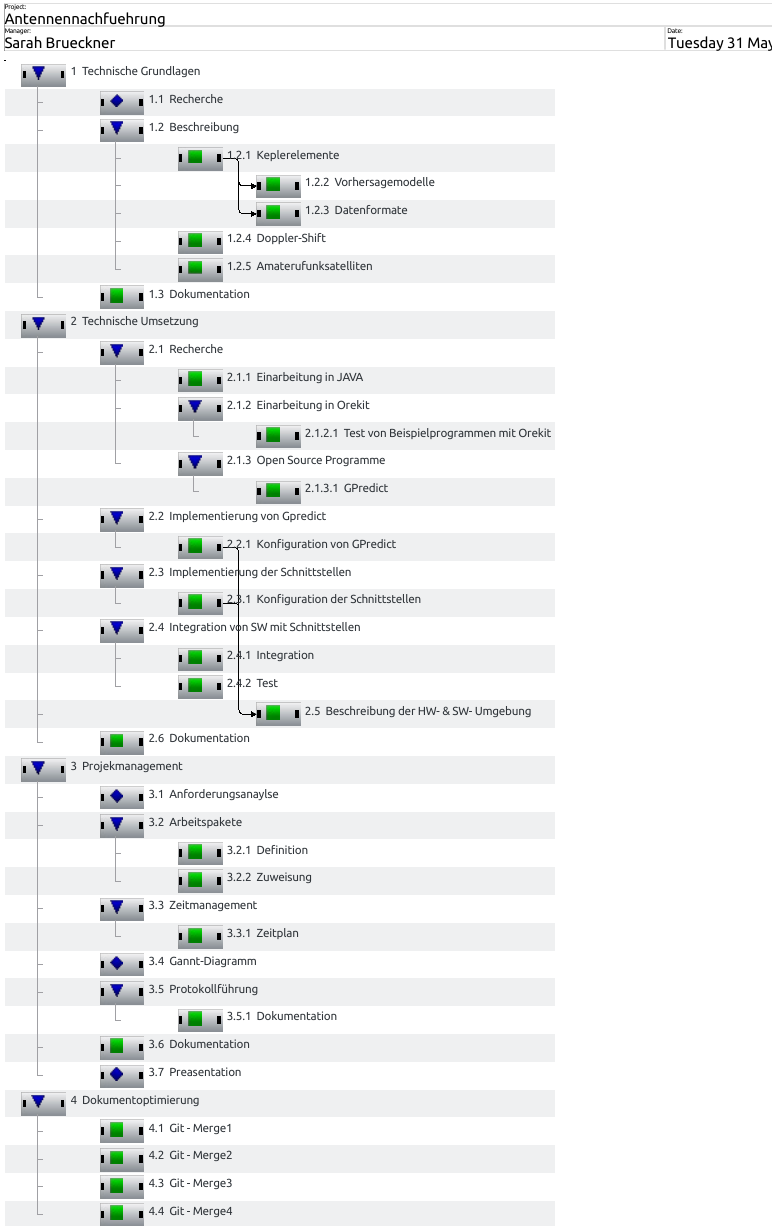
\includegraphics[width=0.6\linewidth]{./images/Tasks}
\caption{Projektstrukturplan}
 \label{fig:projektstruktur}
\end{figure}
\\
Die Studienarbeit ist in vier Themen aufgeteilt: Technische Grundlagen, Technische Umsetzung, 
Projektmanagement und Dokumentenoptimierung. Bei dem Thema ``Technische Grundlagen'' soll der 
theoretische Hintergrund beleuchtet werden. Fragen wie, ``Was ist unter den Keplerelemente zu 
verstehen und wie kann aus ihnen Azimut und Elevation bestimmt werden?'', müssen beantwortet 
werden. Diese Beschreibung ist grundlegend zum Verständnis der zu implementierenden Software 
zur Antennennachführung. Das Implementieren der Software wird in der ``Technischen Umsetzung'' 
durchgeführt. Dabei muss im ersten Schritt eine geeignete Software validiert werden. Die 
Implementierung setzt auch das Wissen über die Hard- und Softwareumgebung voraus, welche zu 
verwenden sind. Es folgt die Konfiguration und Tests der geeigneten Software mit den definierten 
Schnittstellen.
\newpar
Das Projektmanagement definiert die einzelnen Teilaufgaben und koordiniert diese in einem zeitlich 
festgelegten Rahmen um zu einem ergebnisorientierten Projektabschluss zu gelangen. Dabei ist auch 
das Erstellen einer Präsentation Teilaufgabe des Projektmanagements.
\newpar
Für die schriftliche Ausarbeitung dieser Studienarbeit ist eine fortlaufende Dokumentenoptimierung 
nötig um das Arbeiten von drei Studierenden an einem Dokument zu ermöglichen. Zur verteilten 
Versionsverwaltung wird das freie Softwaretool ``Git'' verwendet. Je vier Termine zu einem 
``Merge'' (engl., Zusammenführen) werden zur Versionsverwaltung genutzt und dabei Änderungen von 
Formatierung oder Ähnliches diskutiert.
\newpar
In der folgenden Grafik \ref{fig:arbeitspaket} sind alle für die Studienarbeit benötigten 
Arbeitspakete mit Titel (Name), Verantwortlichem (Responisble), Zuweisung (Allocation) und 
Arbeitszeit (Estimate) aufgeführt.
\begin{figure}[t]
 \centering
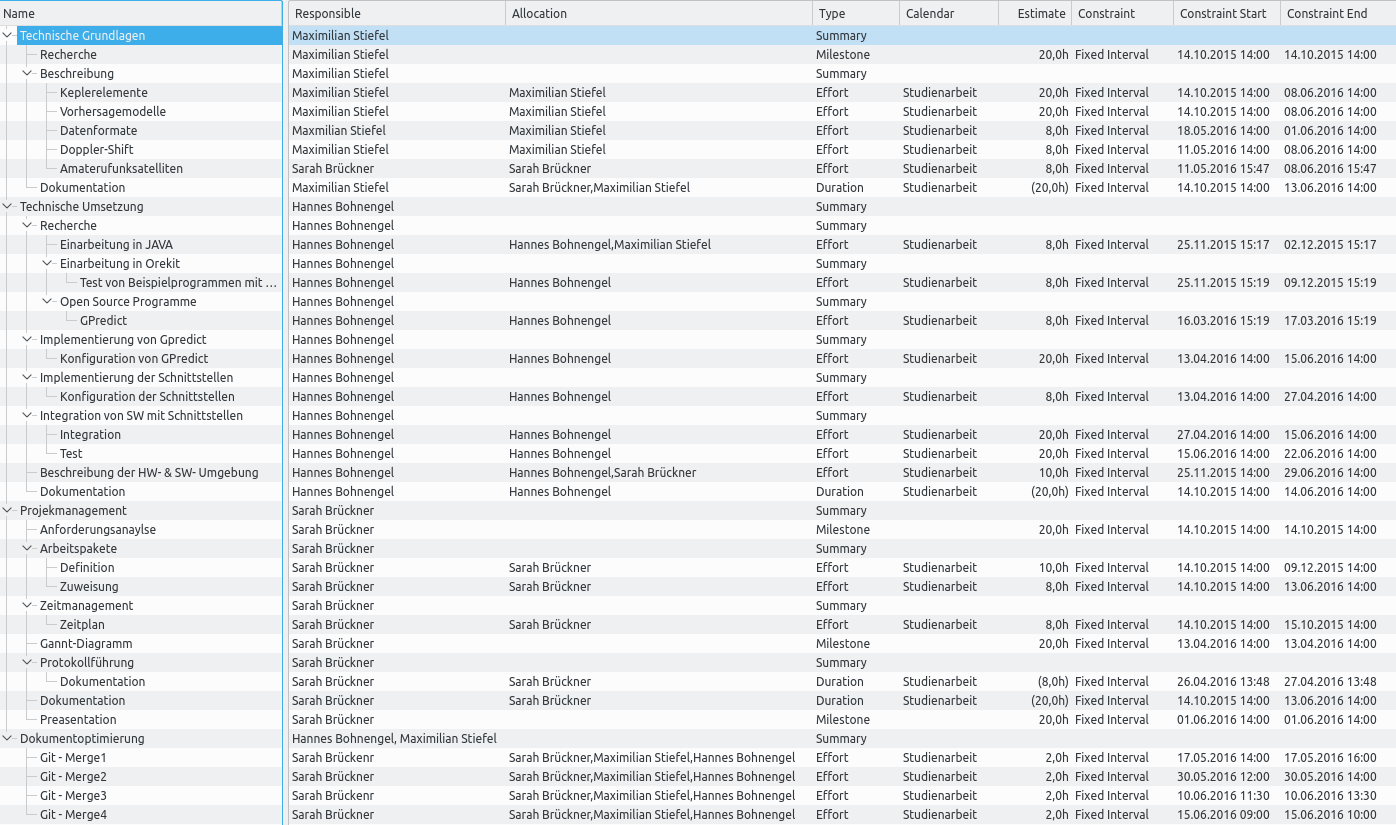
\includegraphics[width=1.0\linewidth]{./images/02depencies}
\caption{Arbeitspakete}
 \label{fig:arbeitspaket}
\end{figure}
